\chapter{Definitions}
\label{chapter-definitions}

TODO we shall introduce a number of definitions, some only auxiliary, some necessary in the whole work

\section{XML Tree}

We shall use the representation introduced in \cite{fidax}, where an XML file is represented by a labeled tree consisting of nodes for elements, attributes and simple text data. This tree shall be called an \textit{XML tree}. For a given node $v$ of an XML tree we define $label(v)$ (name of the node in in the document, only for elements and attributes), $id(v)$ (unique identifier across the document) and $value(v)$ (text content, only for attributes and simple text data) in the same way as the referenced article does.

Without a loss of generality we ignore the actual ordering of nodes in the tree.

\paragraph{Example}

This example introduces an XML file fragment that will be used for demonstration throughout this work. XML tree representing it is in Figure \ref{image-definitions-example-xml-tree}, where each node is annotated with a triple $label(v) : id(v) : value(v)$.

\begin{verbatim}
<x>
  <y a="1" b="2"/>
  <y a="3" c="4"/>
  <y/>
  <z a="1"/>
</x>
\end{verbatim}

\begin{figure}
  \caption{Example XML Tree}
  \label{image-definitions-example-xml-tree}
  \centering
    \subfigure[XML tree]{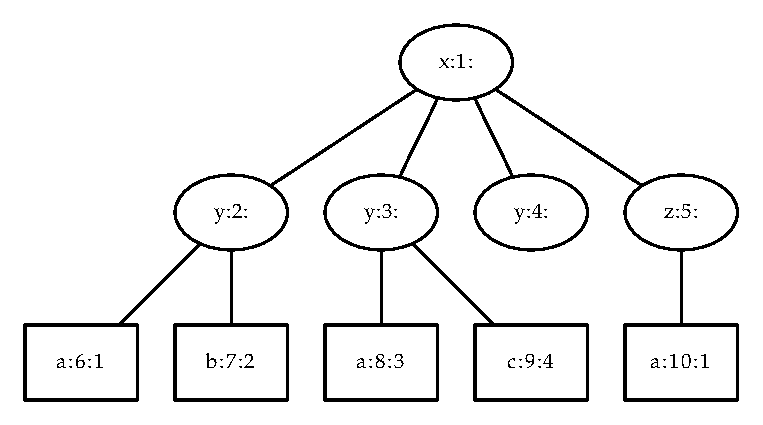
\includegraphics[width=.45\textwidth]{images/definitions/xml-tree}}
    \subfigure[Attribute mappings]{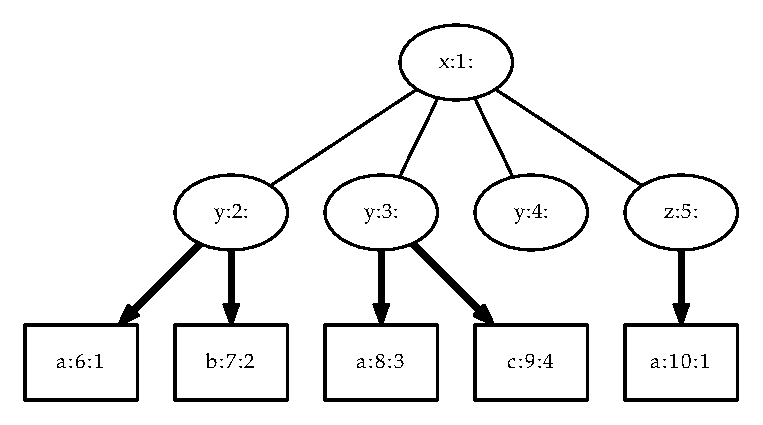
\includegraphics[width=.45\textwidth]{images/definitions/xml-tree-ams}}
\end{figure}

Furthermore, we denote $\mathcal{I}$ the set of all ids and $\mathcal{V}$ the set of all values in the document. We will need two more definitions from the article.

\begin{define}[Node equality]
	$v_1$ and $v_2$ are node equal, written $v_1 =_n v_2$ iff $id(v_1) = id(v_2)$.
\end{define}

\begin{define}[Value equality]
	$v_1$ and $v_2$ are value equal, written $v_1 =_v v_2$ iff $value(v_1) = value(v_2)$.
\end{define}

\section{ID, IDREF, IDREFS Attributes}
\label{section-definitions-id-attributes}

According to \cite{Bray:08:EML}, an XML attribute may have the type \textit{ID}, \textit{IDREF} or \textit{IDREFS} (among others). Following constraints are related to these types.

\begin{quote}
\textbf{Validity constraint: ID}

Values of type \textbf{ID} \textsc{must} match the Name production. A name \textsc{must not} appear more than once in an XML document as a value of this type; i.e., \textbf{ID} values \textsc{must} uniquely identify the elements which bear them.

\textbf{Validity constraint: One ID per Element Type}

An element type \textsc{must not} have more than one \textbf{ID} attribute specified.

\textbf{Validity constraint: ID Attribute Default}

An \textbf{ID} attribute \textsc{must} have a declared default of \textbf{\#IMPLIED} or \textbf{\#REQUIRED}.

\textbf{Validity constraint: IDREF}

Values of type \textbf{IDREF} \textsc{must} match the Name production, and values of type \textbf{IDREFS} \textsc{must} match Names; each Name \textsc{must} match the value of an \textbf{ID} attribute on some element in the XML document; i.e. \textbf{IDREF} values \textsc{must} match the value of some ID attribute.
\end{quote}

%\section{XML Keys} - is this necessary at all?

%TODO

%\subsection{According to Specification}

%TODO compare them to ID attributes

%\subsection{According to \cite{keX}}

%TODO show how a XML key is defined using the keX notation % this is a terrible sentence

\section{Attribute Mappings}

Now we return to \cite{fidax} to define the notion of an \textit{attribute mapping} (or AM for short). \nomenclature{AM}{Attribute Mapping}
We will use a different definition (without introducing keys from \cite{keX}) that will however give us the same result.

\begin{define}[$\Sigma^E$, $\Sigma^A$, $\Sigma$]
	$\Sigma^E$ is the set of all element labels, $\Sigma^A$ is the set of all attribute labels. $\Sigma = \Sigma^E \cup \Sigma^A$ is their union and effectively the set of all labels in the document (simple text data nodes do not have a label).
\end{define}

\begin{define}[Attribute mapping]
	For $x \in \Sigma^E$ and $y \in \Sigma^A$ we define the \textit{attribute mapping} of y over x, denoted $M_{x}^{y}$, the $\mathcal{I} \times \mathcal{I}$ relation defined by
	\[M_{x}^{y} = \{ (z,w): label(z) = x, label(w) = y, parent(w) = z \}\]
\end{define}

Thus the relation $M_{x}^{y}$ contains edges in the XML tree connecting element nodes labeled $x$ and attribute nodes labeled $y$.

We can use projection to retrieve all the unique \textit{ids} of either elements or attributes from the relation, with notation $\pi_E(M_{x}^{y})$ and $\pi_A(M_{x}^{y})$.

\begin{define}[Type of the attribute mapping]
	Attribute mapping $M_{x}^{y}$ is of the \textit{type} $\tau(M_{x}^{y}) = x$.
\end{define}

\paragraph{Example}
The XML tree from Figure \ref{image-definitions-example-xml-tree} has the following non-empty AMs drawn in bold lines: $M_{y}^{a} = \{(2,6), (3,8)\}$, $M_{y}^{b} = \{(2,7)\}$, $M_{y}^{c} = \{(3,9)\}$ and $M_{z}^{a} = \{(5,10)\}$.

Following example equations hold.
\begin{eqnarray*}
\pi_E(M_{y}^{a}) & = & \{2, 3\} \\
\pi_A(M_{z}^{a}) & = & \{10\} \\
\tau(M_{y}^{c}) & = & y
\end{eqnarray*}

\begin{define}[Image of the attribute mapping]
	\textit{Image} $\iota$ of the attribute mapping $M_{x}^{y}$ is defined as $\iota(M_{x}^{y}) = \{z: z = value(w), w \in \pi_A(M_{x}^{y})\}$
\end{define}

So the image of an AM is a set of all the values of all the attribute nodes contained in the mapping.

\paragraph{Example}
Again referring to the XML tree from \ref{image-definitions-example-xml-tree}, we get the following AM images.
\begin{eqnarray*}
\iota(M_{y}^{a}) & = & \{1, 3\} \\
\iota(M_{y}^{b}) & = & \{2\} \\
\iota(M_{y}^{c}) & = & \{4\} \\
\iota(M_{z}^{a}) & = & \{1\} \\
\end{eqnarray*}

\paragraph{Attribute Mapping Model}
An attribute mapping model is a data structure containing the information about all the AMs in a document, together with their images. We shall use this notion later in experimental part of this work.

\section{ID Set}
\label{section-definitions-id-set}

Based on the requirements for an ID attribute from Section \ref{section-definitions-id-attributes} we will define ID set with the help of the following definition.

\begin{define}[Candidate attribute mapping]
An attribute mapping $m$ is a \textit{candidate attribute mapping} if it is an injective function, that is,
\[|m| = |\pi_E(m)| = |\pi_A(m)| = |\iota(m)|\]
\end{define}

\paragraph{Example}
In our example all the attribute mappings are candidate AMs.

Now we can proceed to define an ID set.

\begin{define}[ID set]
A set of candidate attribute mappings $I = \{m_1, \ldots m_n\}$ is an \textit{ID set} iff
\[\bigcap_{m_i \in I} \tau(m_i) = \emptyset \wedge \bigcap_{m_i \in I} \iota(m_i) = \emptyset\]
\end{define}

That is, an ID set has images without repeating values and all the types are unique (an element cannot have more than one ID attribute).

\paragraph{Example}
Returning to our example, the following are all the possible ID sets: $\{ M_{y}^{a} \}, \{ M_{y}^{b} \}, \{ M_{y}^{b}, M_{z}^{a} \}, \{ M_{y}^{c} \}, \{ M_{y}^{c}, M_{z}^{a} \}$. Note that once we select an AM of type $y$ we can never add any other with the same type. Note also that $\{ M_{y}^{c}, M_{z}^{a} \}$ is not an ID set, because $\iota(M_{y}^{c}) \cap \iota(M_{z}^{a}) \neq \emptyset$.

\subsection{IDREF and IDREFS Condition}

Given an ID set $I$, the requirements from Section \ref{section-definitions-id-attributes} give us the following condition for an attribute mapping $m$ to be marked IDREF.
\[\iota(m) \subseteq \bigcup_{m_i \in I} \iota(m_i)\]
Furthermore if $m$ contains multivalued attributes, it is to be marked IDREFS.

\section{Attribute Mapping Weight}
\label{section-definitions-weight}

This definition of weight for AMs or AM sets comes from \cite{fidax} again.

Let $M = \{m_1, \dots m_i\}$ be the set of all non-empty AMs in the document.

\subsection{Support}

\begin{define}[Support]
\textit{Support} of an attribute mapping $m$ is defined as follows.
\[\phi(m) = \frac{|m|}{\sum_{p \in M}|p|}\]
\end{define}

From the cited article:
\begin{quote}
The support of attribute mapping $M_x^y$ is the fraction of edges in the XML tree that connect $x$ elements to $y$ attributes.
\end{quote}

\paragraph{Example}
Support of $M_{y}^{a}$ in our example is $2 / (2+1+1+1) = 0.4$. Support of every other mapping is $1 / (2+1+1+1) = 0.2$.

\subsection{Coverage}

\begin{define}[Coverage]
\textit{Coverage} of an attribute mapping $m$ is defined as follows.
\[\chi(m) = \left( \sum_{p \in M, p \neq m} |\iota(m) \cap \iota(p)| \right) / \sum_{p \in M} |\iota(p)|\]
\end{define}

Again from the article:
\begin{quote}
The coverage of an attribute mapping measures how much of the image of that mapping occurs elsewhere, as a fraction of all mappings images in the document.
\end{quote}

\paragraph{Example}
Coverage of $M_{y}^{a}$ in our example is $(0+0+1) / (2+1+1+1) = 0.2$. Coverage of $M_{z}^{a}$ is $0.2$ as well, all the other mappings have coverage $0$.
\\

\textit{Weight} of an attribute mapping is then defined as a linear combination of its support and coverage.

\begin{define}[Weight]
For $\alpha, \beta \geq 0$ as relative priorities of support and coverage we define the AM \textit{weight} as follows.
\[weight(m) = \alpha . \phi(m) + \beta . \chi(m)\]
For a set of AMs (which may or may not be an ID set) $S = \{m_1, \ldots m_i\}$ we define the weight of this set as the sum of the weights of its AMs.
\[weight(S) = \sum_{m \in S} weight(m)\]
\end{define}

\section{Independent Set}
\label{section-definitions-is}

We shall need the notion of an indepentent set of vertices in a graph and its weighted variant.

\begin{define}[Independent set]
Given an undirected graph $G = (V, E)$, a set of vertices $I \subseteq V$ is an \textit{independent set}, iff the following holds.
\[\forall v_1, v_2 \in I, v_1 \neq v_2: (v_1, v_2) \notin E \]
\end{define}

\begin{define}[Maximum weighted independent set]
Given an undirected graph $G = (V, E)$ and a weight function $w: V \rightarrow \mathbb{R}$, an independent set $I_{max}$ is the \textit{maximum weighted independent set}, iff the following is satisfied.
\[\forall I' \subseteq V, I' \text{is an independent set}: \sum_{v \in I'} w(v) \leqslant \sum_{v in I_{max}} w(v)\]
\end{define}

TODO finding this is NP-hard - cite

\section{Linear Programming}

TODO define LP rigorously

\begin{eqnarray*}
\max_{x} z & = & \mathbf{c}^{\mathrm{T}}\mathbf{x} \\
s.t.\, A\mathbf{x} & \leqslant & \mathbf{b} \\
\mathbf{x} & \geqslant & 0 \\
\end{eqnarray*}
\[
\mathbf{x} =
\begin{bmatrix}
x_1 \\
x_2 \\
\ldots \\
x_n \\
\end{bmatrix},
\mathbf{c} = 
\begin{bmatrix}
c_1 \\
c_2 \\
\ldots \\
c_n \\
\end{bmatrix},
\mathbf{b} =
\begin{bmatrix}
b_1 \\
b_2 \\
\ldots \\
b_m \\
\end{bmatrix}
\]

Where $\mathbf{x}$ is the vector of variables (to be found by the optimization), $\mathbf{b}$ is the vector and $A$ is the accompanying matrix of constraints and $\mathbf{c}$ is the vector of coefficients for the objective function. $\mathbf{x}$ and $\mathbf{c}$ have length $n$, $\mathbf{b}$ has length $m$ and $A$ has dimensions $m \times n$.

Another way to write this formulation is in the following.

\begin{eqnarray*}
\max_{x} z = \sum_{i=1}^{n} c_i x_i \\
s.t.\, a_{11}x_{1} + a_{12}x_{2} + \ldots + a_{1n}x_{n} & \leqslant & b_{1} \\
	   a_{21}x_{1} + a_{22}x_{2} + \ldots + a_{2n}x_{n} & \leqslant & b_{2} \\
	   \ldots \\
	   a_{m1}x_{1} + a_{m2}x_{2} + \ldots + a_{mn}x_{n} & \leqslant & b_{m} \\
	   x_i \geqslant 0, i = 1, \ldots n \\
\end{eqnarray*}

TODO it is possible to formulate minimization function